\chapter{E--pH Diagrams}\label{ch:b1:e-ph-diagrams}

An iron nail left in rain water rusts; the same nail in a strongly basic
solution keeps its shine for weeks. The steel hull of a ship carries
\omterm{def:b1:periodicity:table}{blocks} of zinc that dissolve in its place, and a copper roof turns
green but never disappears. \omterm{def:b1:nernst:couple}{Redox couples} whose potential depends on pH,
precipitation of hydroxides and oxides, acid--base equilibria: all three
act at once, and a single map gathers them. On a graph of potential
against pH, each species of an element gets the region where it is the
stable form; reading the map tells which species survive in water, which
react together, and where a metal corrodes.

\begin{recall}
The \omterm{thm:b1:nernst:nernst}{Nernst equation}, \omterm{def:b1:nernst:electrode-potential}{standard potentials} and the prediction of redox
reactions are in \cref{ch:b1:nernst}; \omterm{def:b1:predominant-reaction:predominance}{predominance diagrams} in
\cref{ch:b1:predominant-reaction}; precipitation thresholds of
hydroxides and \omterm{def:b1:precipitation:existence-domain}{existence domains} of solids in \cref{ch:b1:precipitation}.
All potentials are at \qty{25}{\celsius}, with $RT\ln 10/F = \qty{0.059}{V}$.
\end{recall}

\begin{omfigure}
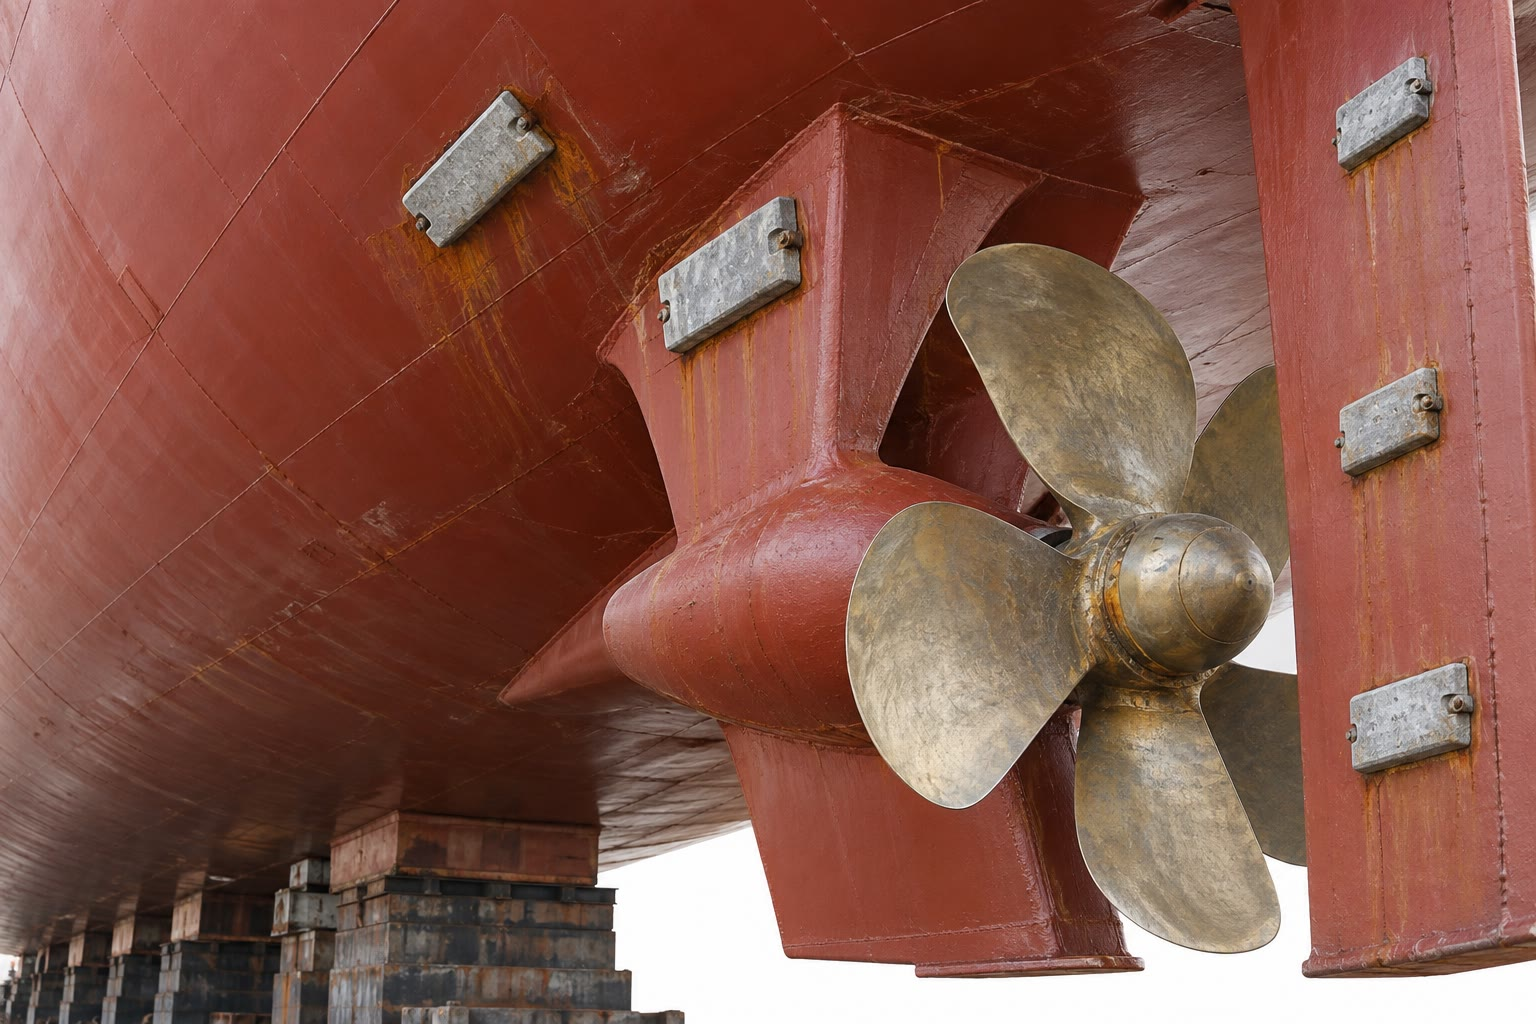
\includegraphics[width=0.6\linewidth]{images/book2/ai/b1-14-ship-anodes.jpg}

{\small The stern of a ship in dry dock. The grey \omterm{def:b1:periodicity:table}{blocks} fixed to the hull
near the propeller are zinc: in sea water they corrode instead of the
steel (\cref{exo:b1:e-ph-diagrams:12}).}
\end{omfigure}

\section{Conventions}

\begin{definition}[Potential--pH diagram, working concentration]\label{def:b1:e-ph-diagrams:e-ph-diagram}
The \emph{potential--pH diagram}\index{potential--pH diagram} of an element
is the plane $(\mathrm{pH}, E)$ divided into regions, each the domain of
predominance (dissolved species) or of existence (solids) of one form of
the element. It is drawn for a chosen \emph{working
concentration}\index{working concentration} $c$, the total concentration
of the element in solution, with these conventions:
\begin{itemize}
  \item on a boundary between two dissolved species, each is at $c$
        (counted in atoms of the element);
  \item on a boundary between a dissolved species and a solid, the
        dissolved species is at $c$ and the solid is just present;
  \item gases are at \qty{1}{bar}.
\end{itemize}
In this chapter $c = \qty{0.010}{mol/L}$.
\end{definition}

The forms of the element are ordered by \omterm{def:b1:nernst:oxidation-number}{oxidation number}: the higher the
number, the higher on the diagram (oxidised forms are stable at high
potential). At a given \omterm{def:b1:nernst:oxidation-number}{oxidation number}, the more basic forms
(hydroxides, oxides, hydroxo \omterm{def:b1:complexation:complex}{complexes}) are to the right.

\begin{proposition}[Slope of a boundary]\label{prop:b1:e-ph-diagrams:boundary-slope}
A boundary between two species of different \omterm{def:b1:nernst:oxidation-number}{oxidation numbers}, whose
\omterm{def:b1:nernst:couple}{half-equation} exchanges $n$ electrons and $m$ protons,
$\mathrm{Ox} + m\,\ce{H+} + n\,\mathrm{e^-} \rightleftharpoons \mathrm{Red} +
\cdots$, is a straight line of slope $-0.059\,m/n$ volt per pH unit. A
boundary between two species of the same \omterm{def:b1:nernst:oxidation-number}{oxidation number} is vertical.
\end{proposition}

\begin{proof}
The \omterm{thm:b1:nernst:nernst}{Nernst equation} gives $E = E^\circ + \frac{0.059}{n}\log\frac{[\mathrm{Ox}]
[\ce{H+}]^m}{[\mathrm{Red}]} = E^\circ + \frac{0.059}{n}\log\frac{[\mathrm{Ox}]}
{[\mathrm{Red}]} - \frac{0.059\,m}{n}\,\mathrm{pH}$, and on the boundary the
concentrations are fixed by the conventions. Two species of the same
\omterm{def:b1:nernst:oxidation-number}{oxidation number} are linked by an acid--base or precipitation equilibrium
without electrons, whose constant fixes the pH of the boundary
whatever the potential.
\end{proof}

\section{Water}

\begin{proposition}[The two lines of water]\label{prop:b1:e-ph-diagrams:water-lines}
Under \qty{1}{bar} of gas, water is reduced to hydrogen below the line
$E = -0.059\,\mathrm{pH}$ and oxidised to oxygen above the line $E = 1.23
- 0.059\,\mathrm{pH}$.
\end{proposition}

\begin{proof}
\ce{2H+ + 2e- -> H2}: $E = 0 + \frac{0.059}{2}\log\frac{[\ce{H+}]^2}{p(\ce{H2})}
= -0.059\,\mathrm{pH}$ at $p = 1$. \ce{O2 + 4H+ + 4e- -> 2H2O}: $E = 1.23 +
\frac{0.059}{4}\log(p(\ce{O2})[\ce{H+}]^4) = 1.23 - 0.059\,\mathrm{pH}$. Below
the first line \ce{H2} is the stable form of the couple (water is
reduced); above the second, \ce{O2} is.
\end{proof}

\begin{definition}[Stability domain of water]\label{def:b1:e-ph-diagrams:water-domain}
The band between the two lines, \qty{1.23}{V} wide at every pH, is the
\emph{stability domain of water}\index{stability domain of water}: a
species whose domain lies entirely inside it neither oxidises nor reduces
water.
\end{definition}

\section{Building a diagram: iron}

\begin{method}[Building a potential--pH diagram]\label{met:b1:e-ph-diagrams:build}
\begin{enumerate}
  \item List the species and sort them by \omterm{def:b1:nernst:oxidation-number}{oxidation number}: for iron,
        \ce{Fe} (0), \ce{Fe^2+} and \ce{Fe(OH)2} ($+$II), \ce{Fe^3+} and
        \ce{Fe(OH)3} ($+$III).
  \item At each \omterm{def:b1:nernst:oxidation-number}{oxidation number}, find the vertical boundaries from the
        precipitation (or acid--base) equilibria at the \omterm{def:b1:e-ph-diagrams:e-ph-diagram}{working
        concentration} (\cref{ch:b1:precipitation}).
  \item For each pair of neighbouring \omterm{def:b1:nernst:oxidation-number}{oxidation numbers}, write the
        \omterm{def:b1:nernst:couple}{half-equation} in each pH range and its \omterm{thm:b1:nernst:nernst}{Nernst equation} with the
        conventions; this gives a straight boundary of known slope.
  \item Assemble the lines from left to right; where three lines meet,
        each continues only on the side where its two species are both
        stable.
  \item Check: the domains must not overlap, and the slopes must agree
        with \cref{prop:b1:e-ph-diagrams:boundary-slope}.
\end{enumerate}
\end{method}

\begin{example}[The iron boundaries]\label{ex:b1:e-ph-diagrams:iron}
With $c = \qty{0.010}{mol/L}$ (and the constants of \cref{ch:b1:precipitation,ch:b1:nernst}):
\begin{itemize}
  \item \ce{Fe^3+}/\ce{Fe(OH)3}: $\mathrm{pH} = 14.00 - \frac13(38.55 - 2) = 1.82$;
        \ce{Fe^2+}/\ce{Fe(OH)2}: $\mathrm{pH} = 14.00 - \frac12(16.31 - 2) = 6.85$.
  \item \ce{Fe^2+}/\ce{Fe}: $E = -0.41 + 0.030\log c = -0.47$~V (pH below 6.85).
  \item \ce{Fe^3+}/\ce{Fe^2+}: $E = 0.77$~V (both at $c$, pH below 1.82).
  \item \ce{Fe(OH)3}/\ce{Fe^2+}: \ce{Fe(OH)3 + 3H+ + e- -> Fe^2+ + 3H2O}, slope
        $-0.177$: $E = 1.09 - 0.177\,\mathrm{pH}$ between pH 1.82 and 6.85.
  \item \ce{Fe(OH)3}/\ce{Fe(OH)2}: one electron, one proton, $E = 0.28 -
        0.059\,\mathrm{pH}$; \ce{Fe(OH)2}/\ce{Fe}: two electrons, two
        protons, $E = -0.07 - 0.059\,\mathrm{pH}$ (pH above 6.85).
\end{itemize}
The intercepts are obtained by continuity at the triple points, or
directly from the Gibbs energies of formation; the diagram below is
computed from the latter, and its boundaries differ from these rounded
values by less than \qty{0.01}{V} or 0.01 pH unit.
% ledger: dfg:Fe2+_ao, dfg:Fe3+_ao, dfg:Fe_OH2_cr, dfg:Fe_OH3_cr, dfg:H2O_l, dfg:OH-_ao (boundaries computed in figdata/bachelor-1/eph-diagrams.py)
\end{example}

\begin{omfigure}
\begin{tikzpicture}
\begin{axis}[
  width=0.8\linewidth, height=8.2cm, xmin=0, xmax=14, ymin=-1.2, ymax=1.6,
  axis x line=bottom, axis y line=left, xlabel={pH}, ylabel={$E$ (V)},
  xtick={0,2,4,6,8,10,12,14}, ytick={-1,-0.5,0,0.5,1,1.5},
  unbounded coords=jump, clip=true,
  tick label style={font=\small}, label style={font=\small}]
\addplot[black!45, dashed] table[x=pH, y=H2] {figdata/out/bachelor-1-eph-diagrams-water.dat};
\addplot[black!45, dashed] table[x=pH, y=O2] {figdata/out/bachelor-1-eph-diagrams-water.dat};
\addplot[omDef, very thick] table[x=pH, y=E] {figdata/out/bachelor-1-eph-diagrams-iron.dat};
\node[font=\small] at (axis cs:3.2,-0.85) {\ce{Fe}};
\node[font=\small] at (axis cs:3.4,0.15) {\ce{Fe^2+}};
\node[font=\small] at (axis cs:0.9,1.45) {\ce{Fe^3+}};
\node[font=\small] at (axis cs:8.5,0.25) {\ce{Fe(OH)3}};
\node[font=\scriptsize] at (axis cs:11.0,-0.56) {\ce{Fe(OH)2}};
\node[font=\scriptsize, black!55, rotate=-14, anchor=south] at (axis cs:12.0,0.52) {\ce{O2}/\ce{H2O}};
\node[font=\scriptsize, black!55, rotate=-14, anchor=south] at (axis cs:2.2,-0.11) {\ce{H2O}/\ce{H2}};
\end{axis}
\end{tikzpicture}

{\small \omterm{def:b1:e-ph-diagrams:e-ph-diagram}{Potential--pH diagram} of iron for $c = \qty{0.010}{mol/L}$ (solid
lines), with the two lines of water (dashed). Every boundary is computed
from tabulated Gibbs energies of formation.}
\end{omfigure}

\section{Copper and zinc}

The same method gives the diagrams of copper (species \ce{Cu}, \ce{Cu+},
\ce{Cu2O} at $+$I, \ce{Cu^2+}, \ce{CuO} at $+$II) and of zinc (\ce{Zn},
\ce{Zn^2+}, \ce{Zn(OH)2}, \ce{Zn(OH)4^2-}). For copper, \ce{CuO}
appears at $\mathrm{pH} = 14.00 - \frac12(20.64 - 2) = 4.68$, and the \ce{Cu+} ion, though listed, has
no domain at all: in acid, $E^\circ(\ce{Cu+}/\ce{Cu}) = 0.52$~V lies above
$E^\circ(\ce{Cu^2+}/\ce{Cu+}) = 0.16$~V, so its would-be domain is
crossed out by the two neighbours (\cref{sec:b1:e-ph-diagrams:reading}).
For zinc, the hydroxide appears at pH 6.81 and redissolves as
\ce{Zn(OH)4^2-} only above 13.97 at this concentration, a sliver at the
right edge.

\begin{omfigure}
\begin{tikzpicture}
\begin{axis}[name=cu,
  width=0.47\linewidth, height=7cm, xmin=0, xmax=14, ymin=-1.4, ymax=1.6,
  axis x line=bottom, axis y line=left, xlabel={pH}, ylabel={$E$ (V)},
  xtick={0,4,8,12}, ytick={-1,-0.5,0,0.5,1,1.5},
  unbounded coords=jump, clip=true,
  tick label style={font=\small}, label style={font=\small}]
\addplot[black!45, dashed] table[x=pH, y=H2] {figdata/out/bachelor-1-eph-diagrams-water.dat};
\addplot[black!45, dashed] table[x=pH, y=O2] {figdata/out/bachelor-1-eph-diagrams-water.dat};
\addplot[omDef, very thick] table[x=pH, y=E] {figdata/out/bachelor-1-eph-diagrams-copper.dat};
\node[font=\small] at (axis cs:5,-0.7) {\ce{Cu}};
\node[font=\small] at (axis cs:2,0.7) {\ce{Cu^2+}};
\node[font=\small] at (axis cs:9.5,0.75) {\ce{CuO}};
\node[font=\scriptsize] (cuo) at (axis cs:11.8,-1.05) {\ce{Cu2O}};
\draw[->, black!70] (cuo.north) -- (axis cs:10,-0.035);
\node[font=\small, anchor=north] at (axis cs:7,1.58) {copper};
\end{axis}
\begin{axis}[at={(cu.east)}, anchor=west, xshift=1.5cm,
  width=0.47\linewidth, height=7cm, xmin=0, xmax=14, ymin=-1.4, ymax=1.6,
  axis x line=bottom, axis y line=left, xlabel={pH}, ylabel={$E$ (V)},
  xtick={0,4,8,12}, ytick={-1,-0.5,0,0.5,1,1.5},
  unbounded coords=jump, clip=true,
  tick label style={font=\small}, label style={font=\small}]
\addplot[black!45, dashed] table[x=pH, y=H2] {figdata/out/bachelor-1-eph-diagrams-water.dat};
\addplot[black!45, dashed] table[x=pH, y=O2] {figdata/out/bachelor-1-eph-diagrams-water.dat};
\addplot[omDef, very thick] table[x=pH, y=E] {figdata/out/bachelor-1-eph-diagrams-zinc.dat};
\node[font=\small] at (axis cs:3.5,-1.15) {\ce{Zn}};
\node[font=\small] at (axis cs:3.2,0.4) {\ce{Zn^2+}};
\node[font=\small] at (axis cs:10.2,0.4) {\ce{Zn(OH)2}};
\draw[->] (axis cs:12.4,1.15) node[left, font=\scriptsize] {\ce{Zn(OH)4^2-}} -- (axis cs:13.95,1.15);
\node[font=\small, anchor=north] at (axis cs:10.5,1.58) {zinc};
\end{axis}
\end{tikzpicture}

{\small \omterm{def:b1:e-ph-diagrams:e-ph-diagram}{Potential--pH diagrams} of copper and zinc ($c =
\qty{0.010}{mol/L}$), with the lines of water (dashed). The domain of
copper metal overlaps the domain of water; that of zinc lies entirely
below the hydrogen line.}
% ledger: dfg:Cu+_ao, dfg:Cu2+_ao, dfg:Cu2O_cr, dfg:CuO_cr, dfg:Zn2+_ao, dfg:Zn_OH2_cr, dfg:Zn_OH42-_ao (boundaries computed in figdata/bachelor-1/eph-diagrams.py)
\end{omfigure}

\section{Reading a diagram}\label{sec:b1:e-ph-diagrams:reading}

\begin{proposition}[Disjoint domains]\label{prop:b1:e-ph-diagrams:disjoint-domains}
If, at a given pH, the domain of an \omterm{def:b1:nernst:couple}{oxidant} lies entirely above that of
a \omterm{def:b1:nernst:couple}{reductant}, with no common part, the two react; species whose domains
share a region can coexist at equilibrium.
\end{proposition}

\begin{proof}
At that pH, above its boundary the \omterm{def:b1:nernst:couple}{oxidant}'s couple has a potential
higher than any the \omterm{def:b1:nernst:couple}{reductant}'s couple can reach: by
\cref{prop:b1:nernst:equilibrium-constant} the reaction between them has
$K > 1$, and it goes on until one of them is used up or their domains
meet. Inside a common region both are the stable forms at the same
potential: nothing drives a reaction.
\end{proof}

Iron and water: the domain of iron metal lies below the line
\ce{H2O}/\ce{H2} at every pH. Iron reduces water, in acid solution with
a visible release of hydrogen; with dissolved oxygen it is oxidised
faster still. Copper: its domain overlaps that of water, so copper does
not reduce water or acids that are not themselves \omterm{def:b1:nernst:couple}{oxidants}, but the
oxygen of air, above it, oxidises it slowly --- the green patina of roofs
is a later product of that oxidation with carbon dioxide and sulfur
compounds. A diagram tells what is possible, not how fast: many reactions
it allows are slow, a question treated in the Year~2 volume.

\begin{definition}[Disproportionation, comproportionation]\label{def:b1:e-ph-diagrams:disproportionation}
\emph{Disproportionation}\index{disproportionation} is the reaction of a
species with itself, one part being oxidised and the other reduced:
\ce{2Cu+ -> Cu^2+ + Cu}. The reverse, two species of the same element
giving one of intermediate \omterm{def:b1:nernst:oxidation-number}{oxidation number}, is
\emph{comproportionation}\index{comproportionation}:
\ce{2Fe^3+ + Fe -> 3Fe^2+}.
\end{definition}

\begin{proposition}[Criterion of disproportionation]\label{prop:b1:e-ph-diagrams:disproportionation-criterion}
A species B of intermediate \omterm{def:b1:nernst:oxidation-number}{oxidation number}, in the couples A/B and
B/C, disproportionates if $E(\mathrm{B}/\mathrm{C}) > E(\mathrm{A}/\mathrm{B})$:
it then has no domain of its own, and a single boundary A/C replaces the
two.
\end{proposition}

\begin{proof}
B is the \omterm{def:b1:nernst:couple}{oxidant} of B/C and the \omterm{def:b1:nernst:couple}{reductant} of A/B. If the B/C couple lies
above A/B, the gamma rule (\cref{met:b1:nernst:predict-redox}) makes B
(\omterm{def:b1:nernst:couple}{oxidant}, upper couple) react with B (\omterm{def:b1:nernst:couple}{reductant}, lower couple), giving C
and A. Geometrically, B would be stable only above $E(\mathrm{B}/\mathrm{C})$
and below $E(\mathrm{A}/\mathrm{B})$, an empty set.
\end{proof}

\begin{definition}[Immunity, corrosion and passivation domains]\label{def:b1:e-ph-diagrams:corrosion-domains}
On the diagram of a metal, the domain of the metal itself is its
\emph{immunity domain}\index{immunity domain} (it cannot be oxidised);
the domains of its dissolved ions form the \emph{corrosion
domain}\index{corrosion domain}; the domains of its solid oxides and
hydroxides, which may coat the metal, form the \emph{passivation
domain}\index{passivation domain}. Whether a coat really protects the
metal is a kinetic matter, treated in the Year~2 volume.
\end{definition}

\begin{method}[Reading a diagram]\label{met:b1:e-ph-diagrams:read}
\begin{enumerate}
  \item Superpose the lines of water: a species whose domain lies outside
        the water band reacts with water (thermodynamically).
  \item For two species of different elements, superpose their diagrams:
        disjoint domains at the pH of interest mean a reaction.
  \item For a metal, locate the point (pH, $E$) of the medium: immunity,
        corrosion or passivation.
  \item Remember that a diagram is drawn for one \omterm{def:b1:e-ph-diagrams:e-ph-diagram}{working concentration};
        the boundaries with dissolved species move by $0.059/n$~V per
        decade of concentration.
\end{enumerate}
\end{method}

Zinc protects iron: in sea water (pH about 8) the zinc and steel of a
hull are in contact; zinc, of lower potential, is oxidised first and
the electrons it releases keep the iron in or near its \omterm{def:b1:e-ph-diagrams:corrosion-domains}{immunity domain}.
The zinc \omterm{def:b1:periodicity:table}{block} is consumed and replaced at each dry dock.

\section{Exercises}

\begin{exercise}[$\star$]\label{exo:b1:e-ph-diagrams:1}
Sort by \omterm{def:b1:nernst:oxidation-number}{oxidation number} of the element the species \ce{Mn}, \ce{Mn^2+},
\ce{MnO2}, \ce{MnO4-}, \ce{Mn(OH)2}, and \ce{Cl-}, \ce{Cl2}, \ce{HClO},
\ce{ClO-}, \ce{ClO3-}.
\end{exercise}

\begin{exercise}[$\star$]\label{exo:b1:e-ph-diagrams:2}
Give the slope of the boundary for each \omterm{def:b1:nernst:couple}{half-equation}:
\ce{Fe(OH)3 + 3H+ + e- -> Fe^2+ + 3H2O}; \ce{2Cu^2+ + H2O + 2e- -> Cu2O + 2H+};
\ce{MnO4- + 8H+ + 5e- -> Mn^2+ + 4H2O}; \ce{Zn(OH)2 + 2H+ + 2e- -> Zn + 2H2O}.
Why does one of them have a positive slope?
\end{exercise}

\begin{exercise}[$\star$]\label{exo:b1:e-ph-diagrams:3}
At what pH do the lines of water pass through 0~V and through
\qty{0.50}{V}? What is the width of the \omterm{def:b1:e-ph-diagrams:water-domain}{stability domain of water} at
pH 7?
\end{exercise}

\begin{exercise}[$\star$]\label{exo:b1:e-ph-diagrams:4}
Using the iron diagram, give the stable form of iron at
(pH 1, $E = 1.0$~V), (pH 4, $E = 0$), (pH 10, $E = -0.4$~V) and
(pH 10, $E = 0.5$~V).
\end{exercise}

\begin{exercise}[$\star\star$]\label{exo:b1:e-ph-diagrams:5}
Recompute the boundary \ce{Fe^2+}/\ce{Fe} and the vertical
\ce{Fe^3+}/\ce{Fe(OH)3} for a \omterm{def:b1:e-ph-diagrams:e-ph-diagram}{working concentration} of
\qty{1.0e-6}{mol/L}, the value used to discuss corrosion. Which domains
grow?
\end{exercise}

\begin{exercise}[$\star\star$]\label{exo:b1:e-ph-diagrams:6}
Derive the boundary \ce{Fe(OH)3}/\ce{Fe^2+}: write the \omterm{def:b1:nernst:couple}{half-equation}, its
\omterm{thm:b1:nernst:nernst}{Nernst equation}, and use continuity at pH 1.82 to show that $E = 1.09 -
0.177\,\mathrm{pH}$.
\end{exercise}

\begin{exercise}[$\star\star$]\label{exo:b1:e-ph-diagrams:7}
Show with the table of \omterm{def:b1:nernst:electrode-potential}{standard potentials} that \ce{Cu+} disproportionates
at pH 0 and give the potential of the single boundary \ce{Cu^2+}/\ce{Cu}
at $c = \qty{0.010}{mol/L}$.
\end{exercise}

\begin{exercise}[$\star\star$]\label{exo:b1:e-ph-diagrams:8}
Does copper dissolve in hydrochloric acid at pH 0 without air? in nitric
acid (couple \ce{NO3-}/\ce{NO}, $E^\circ = 0.96$~V)? Justify with the
diagram and the potentials.
\end{exercise}

\begin{exercise}[$\star\star$]\label{exo:b1:e-ph-diagrams:9}
Iron(II) solutions left in air turn yellow-brown. Explain with the iron
diagram and the line \ce{O2}/\ce{H2O}, and write the reaction at pH 3.
\end{exercise}

\begin{exercise}[$\star\star\star$]\label{exo:b1:e-ph-diagrams:10}
Build the diagram of zinc for $c = \qty{0.010}{mol/L}$: compute the
vertical boundaries at pH 6.81 and 13.97, the boundary \ce{Zn^2+}/\ce{Zn},
and the equations of \ce{Zn(OH)2}/\ce{Zn} and \ce{Zn(OH)4^2-}/\ce{Zn}.
\end{exercise}

\begin{exercise}[$\star\star\star$]\label{exo:b1:e-ph-diagrams:11}
Superpose the diagrams of iron and of water and discuss the fate of an
iron nail in deoxygenated water at pH 2, at pH 7 and at pH 13. What
changes with dissolved oxygen?
\end{exercise}

\begin{exercise}[$\star\star\star$]\label{exo:b1:e-ph-diagrams:12}
Sacrificial \omterm{def:b1:nernst:cell}{anodes}. A steel hull in sea water (pH 8) is joined to a zinc
\omterm{def:b1:periodicity:table}{block}. Using the diagrams, explain which metal is oxidised, write the
reactions with dissolved oxygen, and say why magnesium would also work
and copper would make things worse.
\end{exercise}

\section{Problem: Bleach and the Pool}

\begin{problem}[{Weekend problem --- \omterm{def:b1:nernst:oxidation-number}{oxidation numbers} of chlorine, the
acid--base pair HClO/ClO\textsuperscript{$-$}, the \omterm{def:b1:e-ph-diagrams:e-ph-diagram}{potential--pH diagram}
of chlorine, and the pH above which dissolved chlorine disproportionates}]
\label{pb:b1:e-ph-diagrams:1}
Bleach is a basic solution of sodium hypochlorite and sodium chloride; a
swimming pool is disinfected by the hypochlorous acid it contains, at a
pH kept a little above 7. Mixing bleach with an acidic cleaner releases
chlorine gas. Data at \qty{25}{\celsius}: $E^\circ(\ce{Cl2(aq)}/\ce{Cl-})
= 1.396$~V, $E^\circ(\ce{HClO}/\ce{Cl2(aq)}) = 1.594$~V,
$\mathrm{p}K_a(\ce{HClO}/\ce{ClO-}) = 7.55$, $RT\ln 10/F = 0.0592$~V;
\omterm{def:b1:e-ph-diagrams:e-ph-diagram}{working concentration} $c = \qty{0.010}{mol/L}$ of chlorine atoms.

\medskip
\noindent\textbf{Part I --- The species.}
\begin{enumerate}
  \item Give the \omterm{def:b1:nernst:oxidation-number}{oxidation number} of chlorine in \ce{Cl-}, \ce{Cl2},
        \ce{HClO} and \ce{ClO-}.
  \item Sort the four species on a vertical axis of \omterm{def:b1:nernst:oxidation-number}{oxidation number}.
  \item Which two species have the same \omterm{def:b1:nernst:oxidation-number}{oxidation number}? How are they
        related?
  \item Write the \omterm{def:b1:nernst:couple}{half-equation} of \ce{Cl2}/\ce{Cl-}.
  \item Write the \omterm{def:b1:nernst:couple}{half-equation} of \ce{HClO}/\ce{Cl2}.
  \item Write the \omterm{def:b1:nernst:couple}{half-equation} of \ce{ClO-}/\ce{Cl-} in basic solution.
\end{enumerate}

\medskip
\noindent\textbf{Part II --- Hypochlorous acid.}
\begin{enumerate}[resume]
  \item Draw the \omterm{def:b1:predominant-reaction:predominance}{predominance diagram} of \ce{HClO} and \ce{ClO-} against
        pH.
  \item Why is their boundary on the \omterm{def:b1:e-ph-diagrams:e-ph-diagram}{potential--pH diagram} vertical?
  \item Compute the fraction of hypochlorous acid at pH 7.4.
  \item Same at pH 8.0. Hypochlorous acid is the better disinfectant: why
        do pool operators keep the pH from drifting up to 8?
  \item In bleach (pH about 12), which form is present?
\end{enumerate}

\medskip
\noindent\textbf{Part III --- The diagram.}
With the conventions of the chapter, \ce{Cl2(aq)} is at $c/2$ and
\ce{Cl-}, \ce{HClO}, \ce{ClO-} at $c$ on a boundary.
\begin{enumerate}[resume]
  \item Show that the boundary \ce{Cl2}/\ce{Cl-} is at $E = 1.396 +
        0.0296\log\bigl((c/2)/c^2\bigr) = 1.446$~V, independent of pH.
  \item Show that the boundary \ce{HClO}/\ce{Cl2} is $E = 1.594 -
        0.0296\log 50 - 0.0592\,\mathrm{pH} \approx 1.544 -
        0.0592\,\mathrm{pH}$.
  \item Find the pH where these two lines cross.
  \item Beyond that pH, the boundary is \ce{HClO}/\ce{Cl-}. Write its
        \omterm{def:b1:nernst:couple}{half-equation} and show that its slope is $-0.0296$.
  \item Compute $E^\circ(\ce{HClO}/\ce{Cl-})$ from the two given potentials.
  \item Write the boundary \ce{ClO-}/\ce{Cl-} above pH 7.55; check its
        continuity at pH 7.55.
  \item Sketch the diagram from pH 0 to 14, with the line \ce{O2}/\ce{H2O}.
  \item Is hypochlorous acid stable in water, thermodynamically? Why does
        a pool still need only small additions of chlorine every day?
\end{enumerate}

\medskip
\noindent\textbf{Part IV --- \omterm{def:b1:e-ph-diagrams:disproportionation}{Disproportionation} and the danger of acid.}
\begin{enumerate}[resume]
  \item Above the pH of question 14, what happens to dissolved chlorine?
        Write the reaction in water and in basic solution.
  \item How is bleach made from chlorine?
  \item Below the same pH, write the reaction between \ce{HClO} and
        \ce{Cl-}. What is it called?
  \item An acidic toilet cleaner brings bleach to pH 1. What happens?
  \item Why is the danger smaller with a weakly acidic product
        (pH 4)? Answer with the diagram, then qualify.
  \item State, to one decimal, the pH above which dissolved chlorine
        disproportionates at $c = \qty{0.010}{mol/L}$.
\end{enumerate}
\end{problem}
